% related work = related scientific articles
% NOT engineering (tsap, at3, tribler-mobile (ppsp-twitter))
% https://scholar.google.nl/scholar?hl=en&q=video+on+demand+android&btnG=&as_sdt=1%2C5&as_sdtp=


\chapter{Introduction}
% 3 to 4 pages with screenshots
% related work in citations in between text

In the era of social media people on earth are more connected then ever before.
%stats

However not every place on earth has an uncensored Internet connection, or has one that can be shut down with the push of a button.
%examples

Although smart phones have brought the Internet into the hands of people, this mobile device is not capable of overturning the power of the Internet-kill-switch, yet.
This is about to change as the self-organising video-on-demand platform Tribler is going to make the jump to mobile devices.
% relevance
A big part of social media is video sharing and streaming.
%stats
There is a great interest in this considering the amount of websites and apps available for streaming video-on-demand services.
%list apps?
Huge video streaming providers like Youtube, Twitch, Periscope, etc. currently dominate the market.
%stats
The problem with those is that none of them are server-less and do not  provide anonymity in any shape or form.
%why

%first point
With servers central to their design they create a single point of failure, even in a decentralized set-up.
Several natural disasters have taken out the necessary infrastructure on numerous occasions for a prolonged period of time.
%examples
Especially in situations like these, people need to communicate and coordinate their efforts to restore safety.
Social media has played a major role in recent calamities when people could mark themselves as safe, effectively broadcasting that information to all their family and friends on social media, instead of contacting them one by one or not at all due to congestion in the communication channels.
So the advantages are obvious, and the vulnerability of central elements underlying current social media too.

%second point
The lack of anonymity becomes a problem when the users privacy is being invaded.
Revealing personal information can be deduced from search queries for example, or associations on social platforms.
When this information can be used for targeted advertising it becomes very valuable, and creates an incentive for the parties that have access to this information to sell it to third parties.
In fact the business model of social media appears to be serving targeted advertisements to its users on behalf of third parties.
What's even worse is social media integrated into regular websites to de-anonymize and track the whereabouts of users even outside of the social media realm.
Whenever users lose control over their privacy it becomes a serious problem.


\chapter{Problem description}
% difficulty or opportunity
% develop software / purchase software / develop non-software solution
% FIRST and scientific, then figures and then filling in the holes


% http://www.internetsociety.org/articles/moving-toward-censorship-free-internet
% https://tools.ietf.org/html/draft-pouwelse-censorfree-scenarios-01#page-4
% http://www.un.org/en/universal-declaration-human-rights/


\begin{figure}[h]
	\centering
	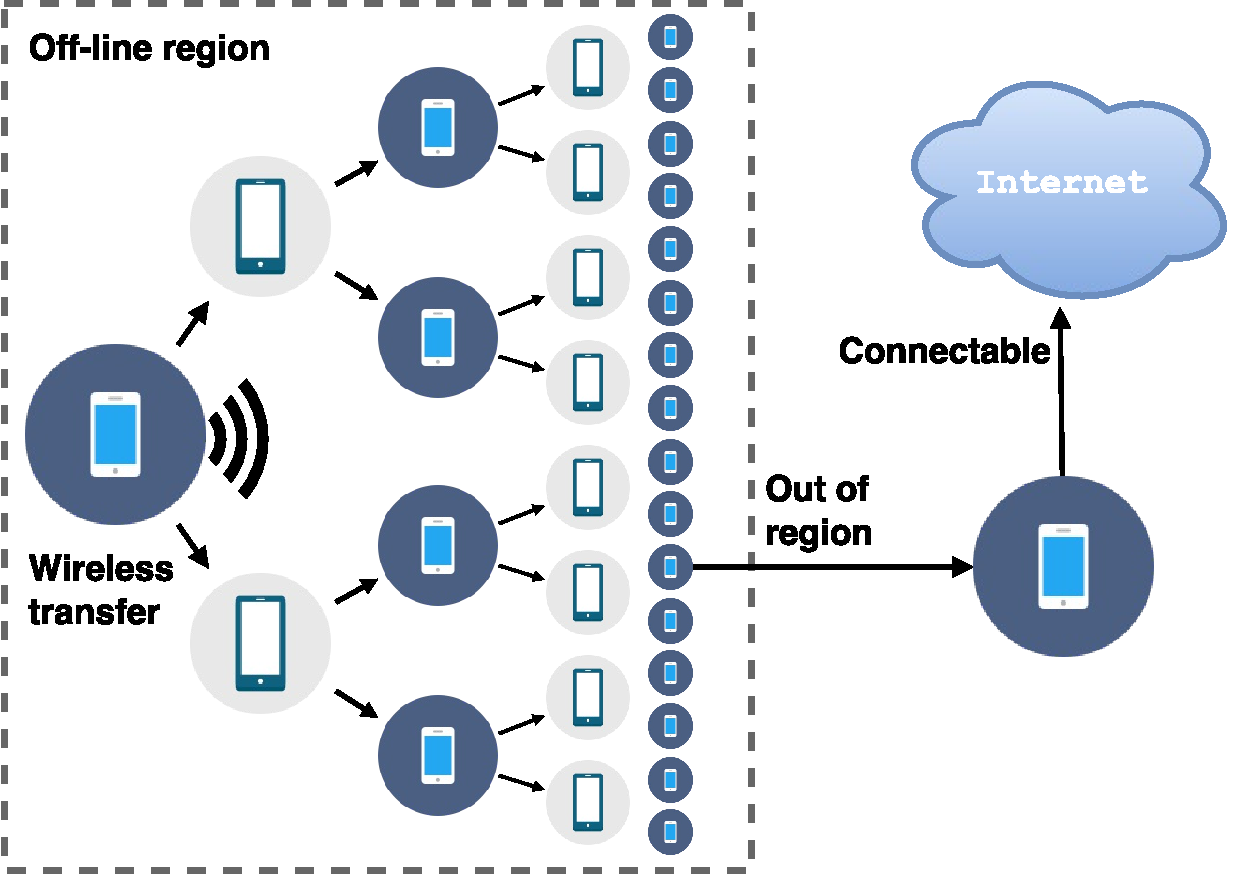
\includegraphics[width=\textwidth]{viral_spreading}
	\caption{Any device can spread to other devices wirelessly.
		Only one device has to travel or connect outside the offline region to make the content connectable to the Internet.}
	\label{fig:viral_spreading}
\end{figure}





\section{Untrusted infrastructure}

Censorship

Partly disconnected

\section{Unavailable infrastructure}

Internet kill-switches

Overloaded

Physically destroyed


The business model of social media directly conflicts with user privacy.
Targeted advertising becomes trivial when the user profile is provided by the user itself with accurate and current information.
When the information is shared with parties outside of the specific social media website it effectively becomes a privacy leak.
Subsequently users will be confronted with their information being misused in various ways, beyond their control.
This lack of control over your own privacy is a problem and can lead to arbitrary interference, possibly even unknowingly. %ref, example, human rights watch, nelie kroes, etc.
The Universal Declaration of Human Rights (UDHR) declares in article 12 that everyone has the right to protection against such interference.

\begin{displayquote}
	No one shall be subjected to arbitrary interference with his privacy, family, home or correspondence, nor to attacks upon his honour and reputation. Everyone has the right to the protection of the law against such interference or attacks.
	(Article 12. UDHR)
\end{displayquote}

Integration of social media on regular websites can easily de-anonymize the visiting user, directly benefiting the business model of targeted advertisements, aggravating this problem.
This incentive not only causes a lack of privacy, but also, paradoxically, a potential lack of freedom of expression.
Every interest and opinion expressed on social media and beyond, whether that is by clicking on anything or publishing videos, is traceable to an individual due to this integration and business model.
If the controlling party of any website connected to social media wants to silence a certain opinion, it can use this connection to trace the individual and any like minded people connected by social interaction.
Particularly on social media do people exercise their right to freedom of opinion and expression.
The UDHR declares in article 19 that everyone has the right to do so without any interference whatsoever.

\begin{displayquote}
	Everyone has the right to freedom of opinion and expression; this right includes freedom to hold opinions without interference and to seek, receive and impart information and ideas through any media and regardless of frontiers.
	(Article 19. UDHR)
\end{displayquote}

%scope
To ensure that no controlling party can exercise censorship we \textbf{distribute authority} over all users, creating an \emph{autonomous} system.
If all information is located in one or a few places, the parties in charge of that location will still have control over it, so we must \textbf{distribute information} over all users, creating a \emph{communication} system.
Then if all users want to use this system to share, order and appreciate each others information, in other words the essence of social media: social interaction, with everyone being able to interact in the same way, we need to  \textbf{distribute functionality} over all users, creating a \emph{cooperation} system.
Fully distributed systems capture these characteristics. %move to solution?
Without any central component in the system it is no longer susceptible to censorship without everyone participating.

Peer-to-peer communication technology is essential for a server-less distributed system.
Mobile devices typically do not require infrastructure to exchange information, like those equipped with Bluetooth or capable of ad hoc Wi-Fi.
Smart phones are ubiquitous everywhere in the world and used to access social media and retrieve information from the Internet.
Fortuitously these are also the type of mobile devices that can communicate peer-to-peer.

\section{Thesis definition}
The main question thus becomes:
How to create a \textbf{self-organising} \textbf{video-on-demand} platform that is \textbf{attack-resilient} and can \textbf{operate autonomously} on a \textbf{mobile device}?

Self-organising in the sense that the platform coordinates the exchange of videos and meta-data fully automatically.

Video-on-demand in the sense that users can simply click and play videos in a streaming fashion, so without waiting for the entire video to be present on the device.

Attack-resilient in the sense that:
First: censorship does not have an effect if the majority of users does not cooperate with the censor.
Second: the privacy of users remains protected while they actively participate on the platform
Third: no network infrastructure required for viral spreading of the entire video platform.

Autonomous operation in the sense that users do not have to manage any files or configuration manually at all to be active on the platform.

Mobile device in the sense that it is low-powered and portable including the network interface and power supply.

These properties will ensure social media with resilience against Internet kill switches, natural disasters and censorship.



\section{Research Limitations} %project scope
% broad / narrow scope, scope of other system()s)
% sub-problems
% ultimate high-level goal
Software development / technical aspect only
Not policy making, organisational perspective, decision making, normative, ethical,
Time limit of 9 months



%LEESWIJZER


